% Figure: the two readings of the cascade property (semigroup vs hemigroup). Referenced from
% §3.4. Pure TikZ, no external file. Paper I's fig-cascade with this article's letters
% (scales r <= s <= t, the ratio lambda): the pedagogic point is the same, one per panel ---
% (a) semigroup increments are indexed by an AMOUNT of scale, (b) hemigroup increments by
% INTERVALS of the scale axis; composition is the shared content.

\begin{figure}[!htb]
\centering
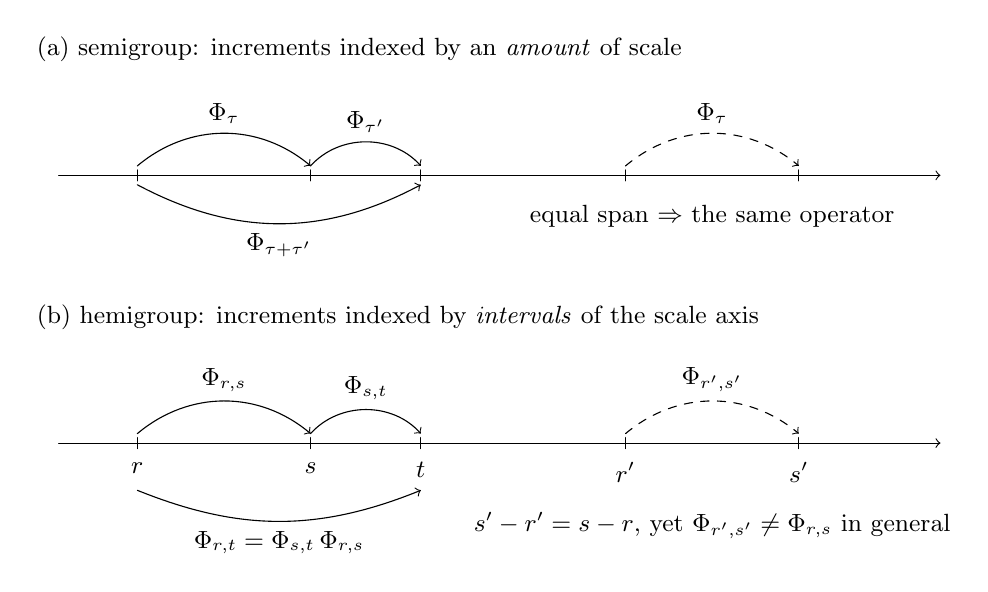
\begin{tikzpicture}[every node/.style={font=\small}, line cap=round]

% ---------- panel (a): semigroup ----------
\begin{scope}[yshift=0cm]
  \node[anchor=west] at (-0.4,1.6) {(a) semigroup: increments indexed by an \emph{amount} of scale};
  \draw[->] (0,0) -- (11.2,0);
  \foreach \x in {1,3.2,4.6,7.2,9.4} \draw (\x,0.07) -- (\x,-0.07);
  \draw[->] (1,0.12) to[bend left=40] node[above] {$\Phi_{\tau}$} (3.2,0.12);
  \draw[->] (3.2,0.12) to[bend left=48] node[above] {$\Phi_{\tau'}$} (4.6,0.12);
  \draw[->] (1,-0.12) to[bend right=28] node[below] {$\Phi_{\tau+\tau'}$} (4.6,-0.12);
  \draw[->,dashed] (7.2,0.12) to[bend left=40] node[above] {$\Phi_{\tau}$} (9.4,0.12);
  \node[anchor=north] at (8.3,-0.25) {equal span $\Rightarrow$ the same operator};
\end{scope}

% ---------- panel (b): hemigroup ----------
\begin{scope}[yshift=-3.4cm]
  \node[anchor=west] at (-0.4,1.6) {(b) hemigroup: increments indexed by \emph{intervals} of the scale axis};
  \draw[->] (0,0) -- (11.2,0);
  \foreach \x/\l in {1/$r$,3.2/$s$,4.6/$t$,7.2/$r'$,9.4/$s'$}
    { \draw (\x,0.07) -- (\x,-0.07); \node[anchor=north] at (\x,-0.12) {\l}; }
  \draw[->] (1,0.12) to[bend left=40] node[above] {$\Phi_{r,s}$} (3.2,0.12);
  \draw[->] (3.2,0.12) to[bend left=48] node[above] {$\Phi_{s,t}$} (4.6,0.12);
  \draw[->] (1,-0.6) to[bend right=22] node[below] {$\Phi_{r,t} = \Phi_{s,t}\,\Phi_{r,s}$} (4.6,-0.6);
  \draw[->,dashed] (7.2,0.12) to[bend left=40] node[above] {$\Phi_{r',s'}$} (9.4,0.12);
  \node[anchor=north] at (8.3,-0.75) {$s'-r' = s-r$, yet $\Phi_{r',s'} \ne \Phi_{r,s}$ in general};
\end{scope}

\end{tikzpicture}
\caption{The two readings of the cascade property. (a)~In the semigroup form the
increment is indexed by an amount of scale: composition adds amounts, and increments of
equal amount are the same operator wherever they act: the axis positions carry no
labels because the operators cannot see them. (b)~In the hemigroup form the increment is
indexed by an interval of the scale axis: composition joins adjacent intervals, and
increments of equal span at different positions need not coincide. The axioms retain what
the two forms share (a measurement of a measurement is a measurement) and drop the
rest.}
\label{fig:cascade}
\end{figure}
